
\section{The Proposed Methodology}

In this section, we first establish the theoretical connection between checkpoint merging and LR decay, formalize our proposed WSM (Warmup-Stable and Merge) schedule, and compare it with the widely used WSD schedule.

\subsection{Theoretical Connection Between LR Decay and Checkpoint Merging}
\label{Theoretical}
The core idea of checkpoint merging in this work is to take an ordered list of checkpoints, $[\theta_n, \theta_{n+1}, \dots, \theta_{n+k}]$, and apply a merge function to generate a single model $\hat{\theta}_{n+k}$. Here, $\theta_i \in \mathbb{R}^d$ represents the model's parameter vector at the $i$-th training iteration.
The most general form is a weighted average of the checkpoints:
\begin{equation}
    \hat{\theta}_{n+k} = \sum_{j=0}^{k} c_j \theta_{n+j}
    \label{eq:weighted_avg}
\end{equation}
where $\{c_j\}$ are non-negative weights that sum to one, i.e., $\sum_{j=0}^{k} c_j = 1$.

This formulation obscures a deeper connection to the training dynamics. We can reveal this connection by expressing each checkpoint in terms of an initial checkpoint $\theta_n$ and the subsequent gradient updates. 
For simplicity, we assume the updates between checkpoints at different time steps are independent and ignore optimizer states. Let $g_{i}$ be the gradient update vector (including the LR) at step $i$, such that the model updates as $\theta_{i+1} = \theta_i - g_i$. Thus, an intermediate checkpoint $\theta_{n+j}$ can be expressed as the sum of an initial state $\theta_n$ and the sequence of negative gradient updates that followed:
\begin{equation}
    \theta_{n+j} = \theta_{n} - \sum_{l=1}^{j} g_{n+l-1}
    \label{eq:theta_as_gradient_sum}
\end{equation}
\begin{figure*}[t]
    \centering
    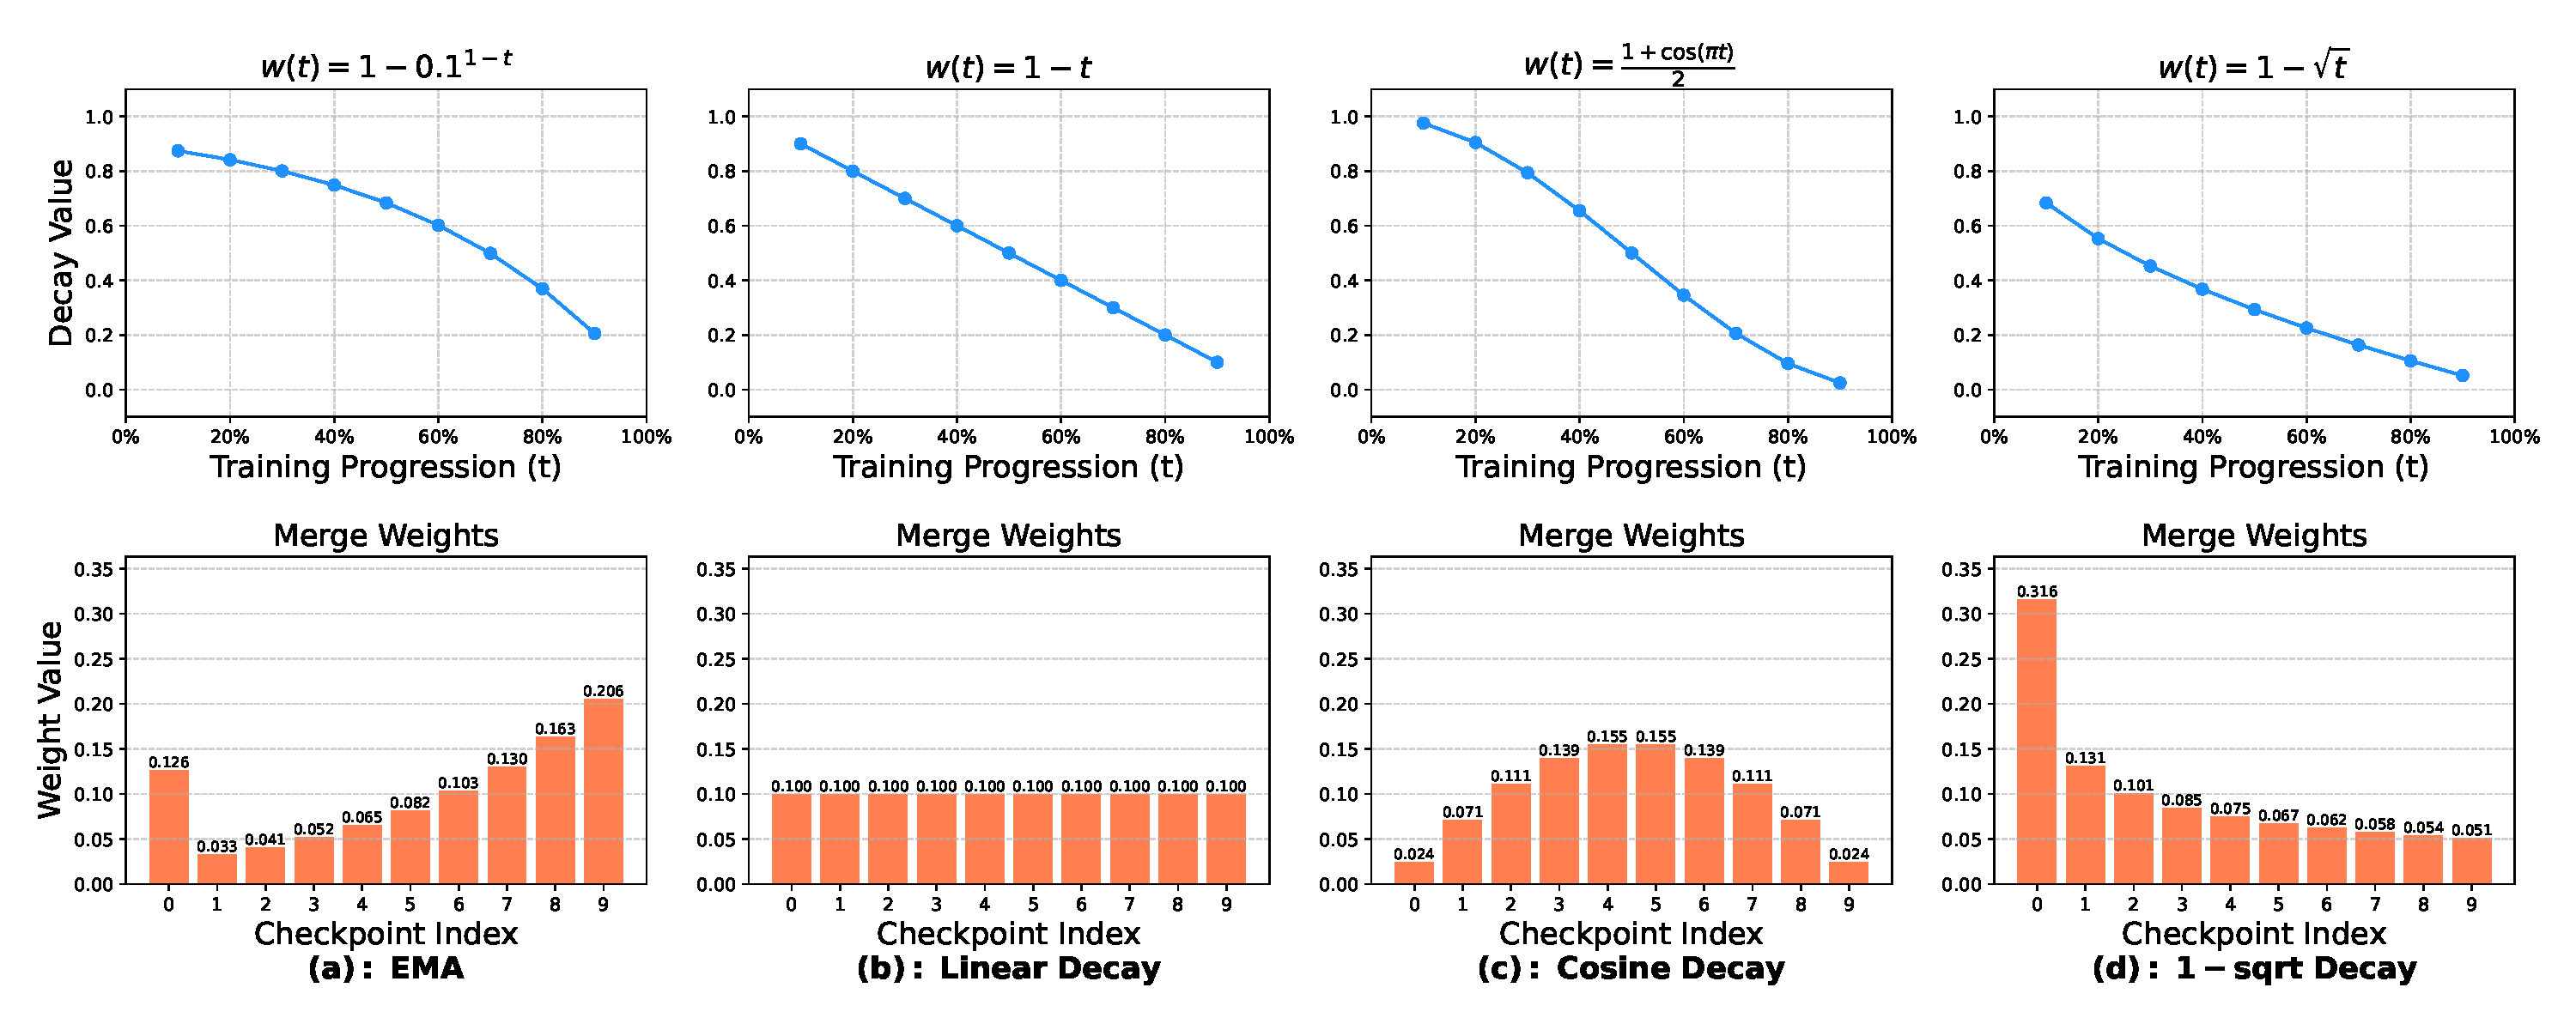
\includegraphics[width=\textwidth]{figs/decay_style_comparison.pdf}
    \caption{\textbf{
    Visualization of checkpoint merging weight distributions and their corresponding decay functions over a span of 10 checkpoints (larger checkpoint indices denote more recent checkpoints).}
(a) Exponential Moving Average (EMA) weights, exhibiting convex decay characteristics;
(b) Uniform averaging weights, demonstrating linear decay behavior;
(c) and (d) Our theoretically derived weights, designed to approximate cosine and 1-{sqrt} decay patterns.
Note: Decay curves are rendered smoothly for clarity, though the underlying weights are applied discretely at each checkpoint.
}
    \label{fig:weight}
\end{figure*}

Furthermore, we can substitute Eq.~\ref{eq:theta_as_gradient_sum} into the general merging formula (Eq. \ref{eq:weighted_avg}) and then rearrange the double summation by changing its order. 
A gradient update $g_{n+i-1}$ is included in the sum for all involved checkpoints $\theta_{n+j}$ where $j \ge i$. 
\begin{align}
    \hat{\theta}_{n+k} &= \sum_{j=0}^{k} c_j \left( \theta_n - \sum_{l=1}^{j} g_{n+l-1} \right) = \theta_n - \sum_{i=1}^{k} \left( \sum_{j=i}^{k} c_j \right) g_{n+i-1} \label{eq:rearrange_sum_step1}
\end{align}
This shows that a weight coefficient of $\sum_{j=i}^{k} c_j$ is applied to the gradient update $g_{n+i-1}$ from step $n+i-1$.
By defining a new set of weights for the gradient updates, $w_i = \sum_{j=i}^{k} c_j$, we arrive at the final equivalent expression for checkpoint merging:
\begin{equation}
    \hat{\theta}_{n+k} = \theta_n - \sum_{i=1}^{k} w_i \cdot g_{n+i-1}
    \label{eq:merge_as_gradient_reweighting}
\end{equation}
This equation shows that merging checkpoints with weights ${c_j}$ is equivalent to applying a synthetic decay schedule defined by weights ${w_i}$ to the gradients accumulated after the base checkpoint $\theta_n$, where a mapping exists between the merge weights ${c_j}$ and the effective learning rates ${w_i}$.
We therefore propose Theorem~\ref{thm:inverse}, which can approximate monotonically decreasing decay curve. Figure~\ref{fig:weight} illustrates various checkpoint merging weights and their corresponding decay curves. Additional proof details are provided in Appendix~\ref{app:Theoretical}.


\begin{theorem}[Checkpoint Weight Derivation from Gradient Decay Schedule]
\label{thm:inverse}
Given a desired sequence of gradient decay coefficients $\{w_i\}_{i=1}^k$ that is monotonically non-increasing and bounded, $1 \ge w_1 \ge w_2 \ge \dots \ge w_k \ge 0$, the corresponding non-negative checkpoint weights $\{c_j\}_{j=0}^k$ required to satisfy Eq. \ref{eq:merge_as_gradient_reweighting} are uniquely determined by:
\begin{equation}
\begin{cases}
    c_k = w_k \\
    c_j = w_j - w_{j+1}, & \text{for } j \in [1, k-1] \\
    c_0 = 1 - \sum_{j=1}^{k} c_j = 1 - w_1
\end{cases}
\label{eq:inverse_formula}
\end{equation}
\end{theorem}


\subsection{Emulating LR Decay through Checkpoint Merging}
The central hypothesis of WSM is that \textit{the optimization benefits of LR decay can be decoupled from the live training process and instead be effectively achieved through the merging of model checkpoints}~\citep{adam,deepseekv3,pma}.
The WSM simplifies the LR schedule by completely eliminating the decay phase:
\[
lr(t) = \begin{cases}
lr_{peak} \cdot \frac{t}{T_{warmup}} & \text{if } t < T_{warmup} \\
lr_{peak} & \text{if } t \ge T_{warmup}  \\
\end{cases}
\]
The WSM pipeline, detailed in Algorithm~\ref{alg:WSM-anneal}, operates in two primary phases. It begins with a standard warmup phase, where the learning rate linearly increases to its peak value, $lr_{peak}$. Following this, the process enters the main stable training phase, where the learning rate is held constant. After a specified step $T_{switch}$, the model can transition from the general pre-training data $D$ to a smaller, high-quality annealing dataset $D_{anneal}$. This allows the ``annealing'' to be focused on a curated data mixture, aligning with practical pre-training methodologies. Throughout this stable phase, checkpoints are periodically saved. Concurrently, an asynchronous merging process continuously fetches the last $n$ checkpoints from storage and combines them into model $W_{merged}$. Specifically, for the $\operatorname{Merge}(\cdot)$ operation, we can select various decay strategies to emulate (e.g., the decay curve shape and minimum LR), calculate the corresponding gradient decay coefficients $\{w_i\}$, and then derive the checkpoint merging weights $\{c_i\}$ based on Theorem \ref{thm:inverse}. This merged checkpoint, which emulates the effect of a decay schedule, provides a robust, annealed model without ever altering the live learning rate.



        
\begin{algorithm}[H] %
\small
\caption{The WSM LRS Pre-training Pipeline}
\label{alg:WSM-anneal}
\begin{algorithmic}
\State \textbf{Input:} Initial model weights $W_0$, pre-training data $D$, high-quality annealing data $D_{anneal}$ (optional), peak LR $lr_{peak}$, warmup steps $T_{warmup}$, switch step $T_{switch}$, checkpointing interval $T_{cpt}$, merging window size $n$
\Statex %
\State \textbf{Initialize:}
\State $\triangleright$ The merged checkpoint.
\State $W_{merged} \gets \text{null}$ 
\State $\triangleright$ Storage for the base (un-merged) checkpoints.
\State $\mathcal{C}_{storage} \gets []$ 
\Statex
\State $\triangleright$ \textbf{Phase 1: Warmup on Pre-training Data}
\For{$t = 1$ to $T_{warmup}$}
    \State $lr(t) \gets lr_{peak} \cdot (t / T_{warmup})$
    \State $W_t \gets \text{Update}(W_{t-1}, D, lr(t))$
\EndFor
\Statex
\State $\triangleright$ \textbf{Phase 2: Stable Training and Merging}
\For{$t = T_{warmup} + 1$ to ...}
    \State $lr(t) \gets lr_{peak}$
    \State $\triangleright$ Select dataset for the current step
    \If{$t > T_{switch}$ \textbf{and} $D_{anneal}$ is available}
        \State $D_{current} \gets D_{anneal}$
    \Else
        \State $D_{current} \gets D$
    \EndIf
    \State $W_t \gets \text{Update}(W_{t-1}, D_{current}, lr(t))$
    \If{$t \pmod{T_{cpt}} == 0$}
        \State $\triangleright$ Save the checkpoint from the main training process.
        \State $\text{SaveToCheckpointStorage}(\mathcal{C}_{storage}, W_t)$
        
        \State $\triangleright$ \textbf{Asynchronously Update the Merged checkpoint}
        \State $C_{latest} \gets \text{GetLastNCheckpoints}(\mathcal{C}_{storage}, n)$
        \If{$\text{len}(C_{latest}) == n$}
            \State  $\triangleright$ Update the merged checkpoint for evaluation.
            \State $W_{merged} \gets \text{Merge}(C_{latest})$ 
        \EndIf
    \EndIf
\EndFor

\State \textbf{return} The stored base checkpoints in $\mathcal{C}_{storage}$ and the merged checkpoint $W_{merged}$.
\end{algorithmic}
\end{algorithm}
\subsection{Discussion}

\paragraph{Choice between offline and online merging}
Initially, we employ an offline, checkpoint-based approach as a powerful exploration framework to discover optimal annealing strategies without impacting the primary training run. By preserving a history of all discrete checkpoints, practitioners can systematically evaluate how different factors influence the final model, including the choice of merging algorithm (simulating various decay curves like linear or cosine) and the annealing duration (by varying the merge window size, $n$). This multi-faceted exploration is impossible with a standard online method, such as an Exponential Moving Average (EMA), which hard-codes a single annealing path into the training process. Crucially, once this offline exploration identifies a superior, fixed strategy (e.g., ``an average of the last 4 checkpoints''), it can then be operationalized as a simple and efficient online process using a sliding window.

\paragraph{Practicality and complexity}
Compared to discovering an optimal decay schedule through multiple, resource-intensive training runs, the merging operations in the WSM strategy save substantial computational resources. The main complexity introduced is storage overhead. For the offline merging approach, which is ideal for exploration, one must store a history of checkpoints, with the total number being the total training tokens divided by the checkpointing interval. However, this is a manageable trade-off, as this storage footprint represents a minor fraction of a typical pre-training budget. Furthermore, once a superior strategy is identified, or in scenarios with extreme storage constraints, an online merging approach can be used. This method minimizes the storage footprint by maintaining only a small, fixed-size window of $n$ checkpoints. Our experiments confirm that a relatively small window (e.g., $n=12$) is sufficient to achieve strong results.

\paragraph{Comparison with \cite{pma}.} 
We notice a concurrent work~\citep{pma} studied model merging in pre-training. We highlight the differences between our work and theirs as follows: 
(1) \textbf{Motivation}: We frame checkpoint merging as a novel LR scheduling mechanism, with the primary goal of discovering a schedule that outperforms strong baselines like WSD. In contrast, their work treats model merging as a standalone pre-training technique, evaluating its value by comparing the performance of the merged model against its before-merge checkpoints.
(2) \textbf{Methodology}: Our approach is theory-driven. We first establish a formal theoretical connection between LR decay and checkpoint merging (Section~\ref{Theoretical}) and then leverage merge weights to simulate various decay curves. They mainly conducts empirical studies of merging algorithms, proposing heuristic methods including WMA, SMA, and EMA. 
(3) \textbf{Key Findings}: Through extensive experiments, we identify the merge duration as the most critical hyperparameter influencing final model performance. Ultimately, our method \textit{surpasses} the performance of WSD-annealed baseline (Section~\ref{sec:main}). In contrast, their work concludes that checkpoint merging can effectively \textit{match} the performance of an annealed model. 
The findings from our work and that of \cite{pma} are complementary, collectively providing practical insights into checkpoint merging for LLM pre-training.


\section{Experiment}
\label{sec:exp}

\subsection{Experiment Setup}
The model we used for the experiment is Ling-mini, a standard MoE model with a total of 16.3 billion parameters and 1.4 billion active parameters. Ling-mini adopts a fine-grained expert configuration, consisting of 1 dense layer and 19 MoE layers. Each MoE layer includes 256 experts, with 8 experts being activated for each token, along with one additional shared expert. We utilized the AdamW optimizer~\citep{adamw}, and the hyperparameters are set to $\beta_1 = 0.9$ and $\beta_2 = 0.95$, with 0.1 weight decay applied. Through preliminary scaling laws experiments, we set the peak LR and batch size to 4.78e-4 and 2048, respectively.

We begin with a checkpoint pretrained on 10.2 trillion tokens total - comprising 10 trillion tokens at standard 4,096 length sequences plus 200 billion long-context tokens - all trained using a stable, constant LR. 
Then, we introduce a specialized high-quality annealing dataset and branch the training into two distinct strategies for an additional 400B tokens to compare their effectiveness:
(1) We apply a conventional LR decay schedule to the model. This branch serves as our baseline, representing the standard Warmup-Stable-Decay (WSD) methodology.
(2) We continue training with the same constant LR. The final model is then produced by merging the checkpoints saved during this stable phase. This branch represents our proposed WSM schedule.
Unless otherwise specified, we save a checkpoint every 25B tokens and use mean averaging to merge the most recent checkpoints.
Comprehensive details regarding our model architecture, specific training parameters, dataset composition, and evaluation protocols are provided in Appendix~\ref{setup}.


\subsection{Overall Performance of WSM Schedule}
\label{sec:main}
\begin{figure*}[t]
    \centering
    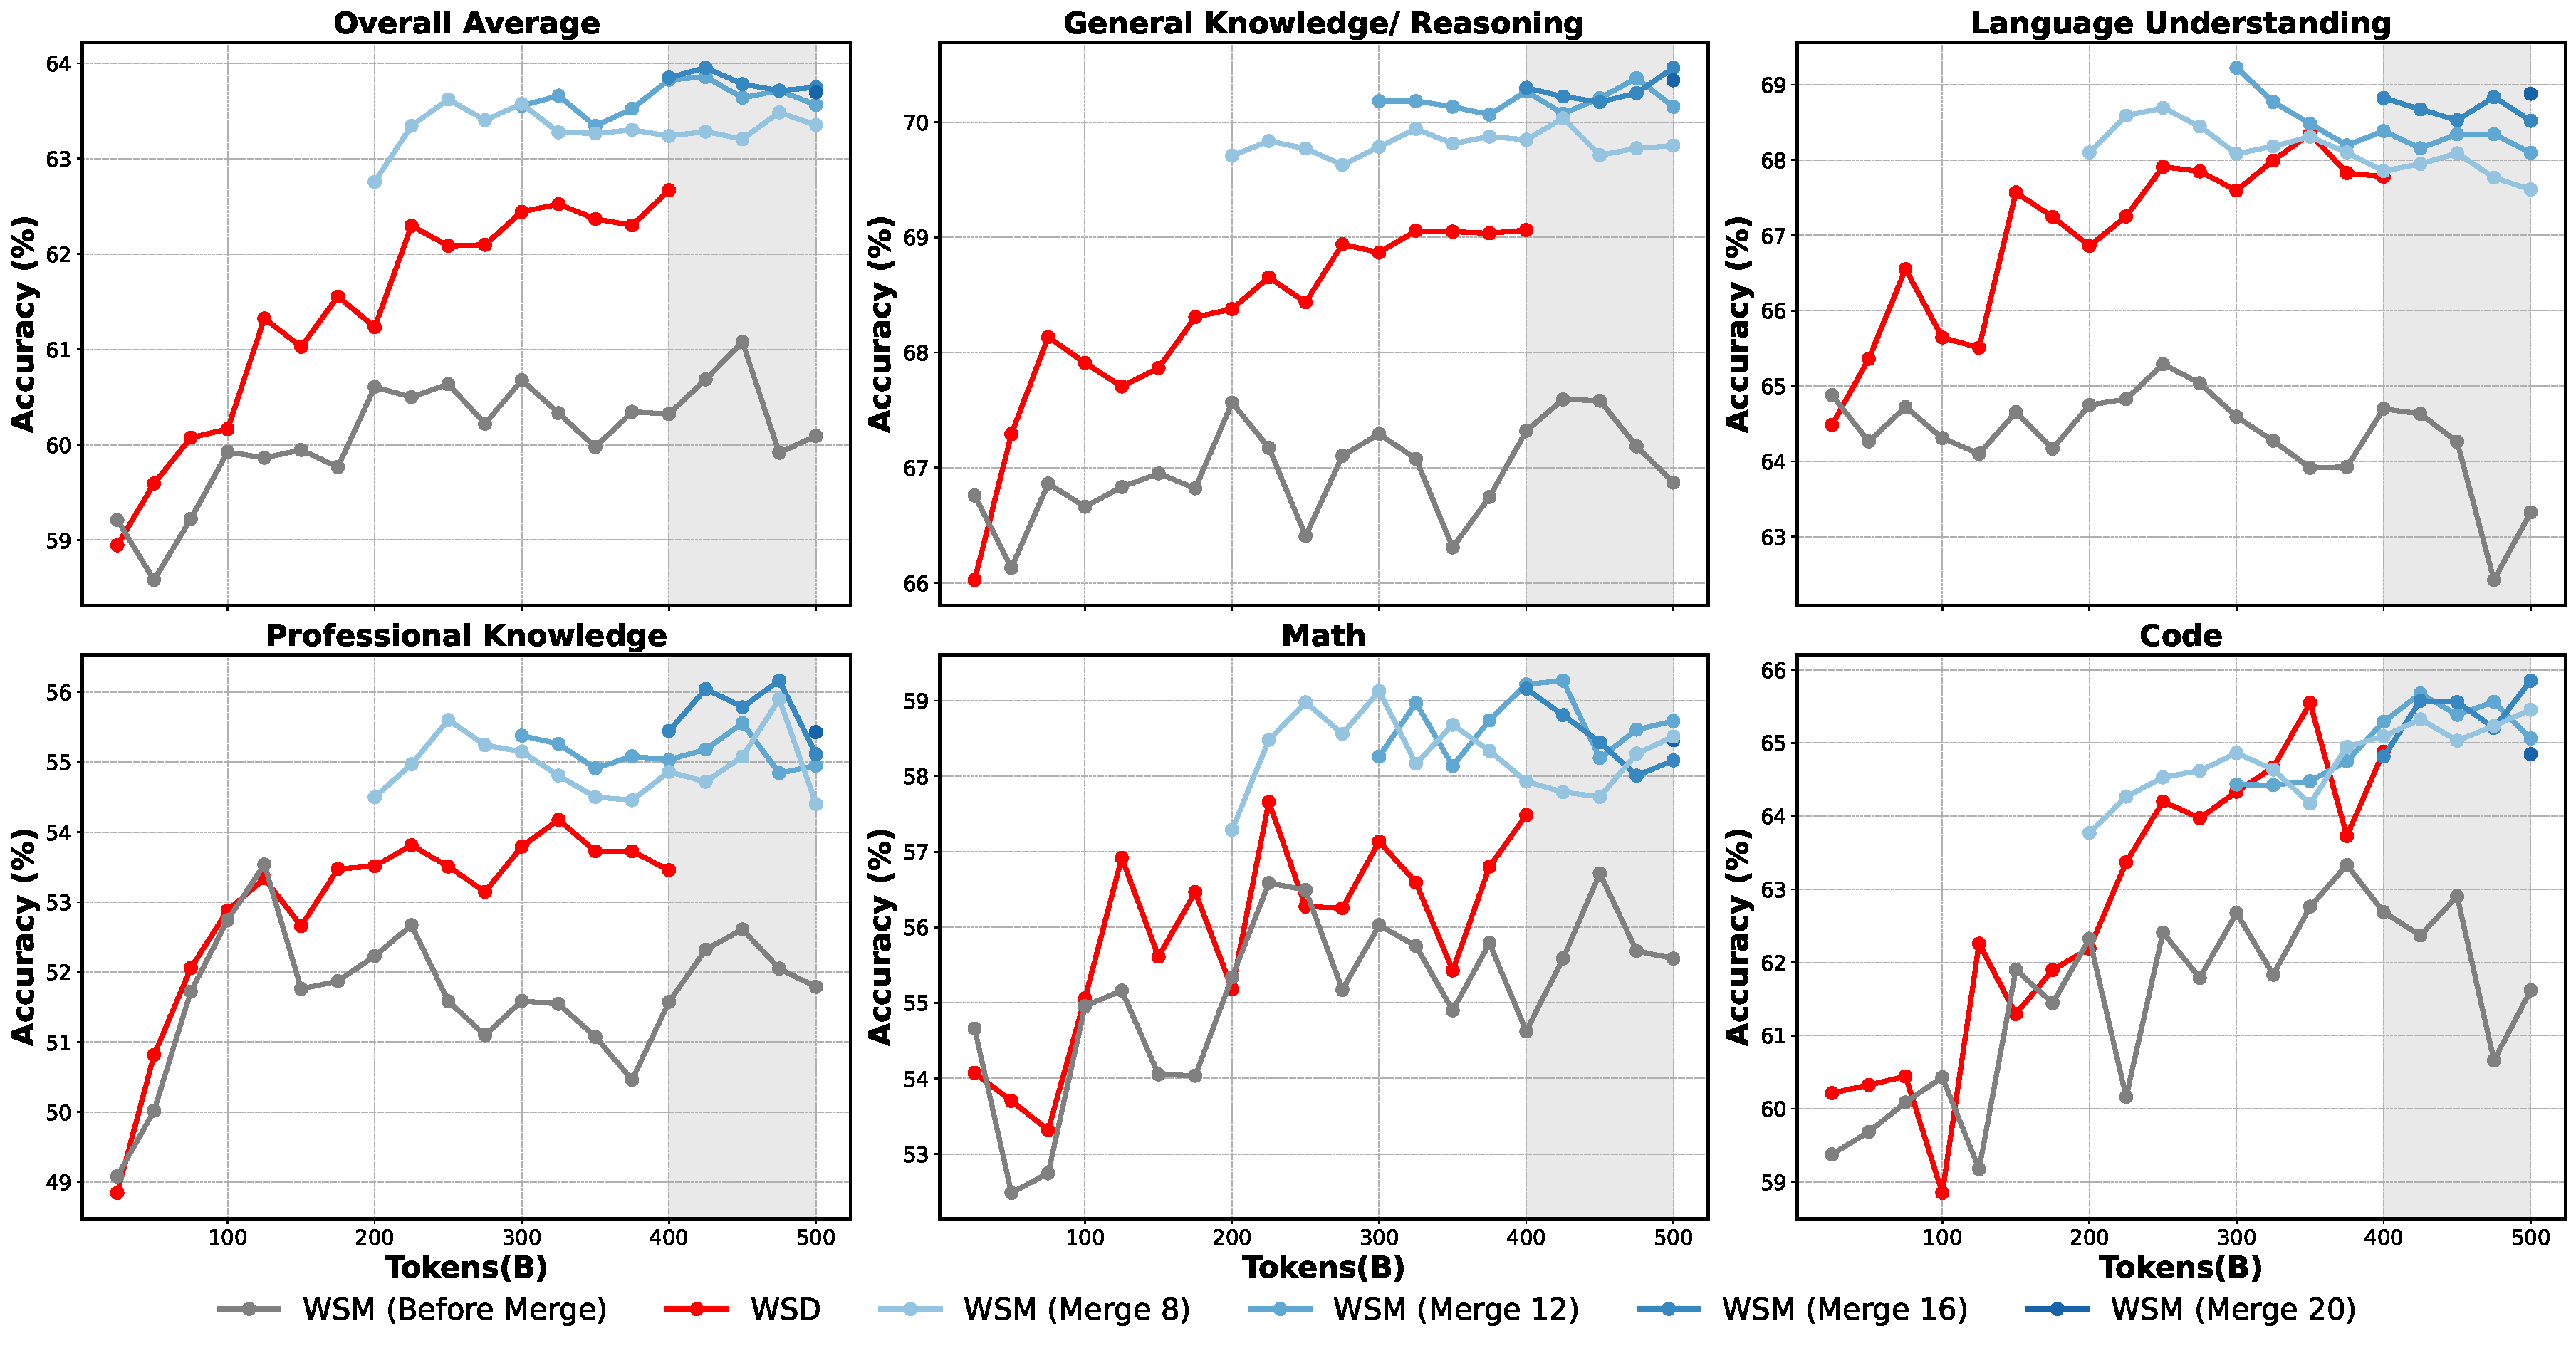
\includegraphics[width=\textwidth]{figs/main.pdf}
    \caption{\textbf{Comprehensive performance comparison (overall and by category) between our WSM schedule (via checkpoint merging) and standard WSD scheduling (via learning rate decay).} Both approaches are initialized from the same pretrained checkpoint (10.2T tokens with constant LR). Notably, while WSD requires predetermined decay strategy (e.g., decay over 400B tokens in this study), WSM eliminates such constraints, enabling seamless training continuation (gray regions) and flexible decay behavior approximation.}
    \label{fig:main}
\end{figure*}

\paragraph{Immediate effects during pre-training }
In this section, we present a comprehensive performance comparison between our proposed WSM schedule and the baseline WSD schedule. We evaluate three series of checkpoints: (1) those obtained using the standard LR decay schedule in WSD, (2) checkpoints from the last stable phase of WSM before merging, and (3) our final merged checkpoints from the WSM method using various merge durations (window sizes). The category-wise average results are summarized in Figure~\ref{fig:main} and Table~\ref{tab:base_model_comparison}, with scores for each benchmark provided in Appendix~\ref{all_datasets}. 

Our first and most significant finding is that the WSM method consistently outperforms WSD across the majority of tasks considered. On average, WSM achieves performance improvements across all benchmark categories.
Notably, when comparing the best-performing checkpoint from each strategy, WSM improves upon WSD by an average of 1.3 points.
We observe remarkable improvements of up to 2.7 points on MATH, 2.4 points on HumanEval, 2.1 points on MMLU-Pro.
These results provide compelling evidence that replacing the LR decay phase used in WSD with the checkpoint merging strategy of WSM is not only a feasible alternative but also a more effective approach for enhancing the diverse capabilities of the final pretrained model.


\paragraph{Long-term implications for post-training}
While WSM demonstrates promising results in the pre-training phase, we further investigate its long-term impact on subsequent post-training stages. We apply supervised fine-tuning on checkpoints generated by the WSM and WSD under identical settings for 5 epochs. Results in Table~\ref{tab:instruct_model_comparison} show that this advantage persists beyond the post-training phase.





\begin{table}[htbp]
  \centering
  \small
  
  \caption{Base model performance comparison. Results are reported based on the checkpoint with the highest average benchmark score.}
  \label{tab:base_model_comparison}
  \begin{tabularx}{\textwidth}{ c l C C C C C c C }
    \toprule
    & & General Knowledge & Language Modeling & Math & Code & Professional Knowledge & & Overall Average \\
    \midrule
    \multirow{3}{*}{Base Model}
    & WSD                & 69.06 & 67.78 & 57.49 & 64.88 & 53.46 & & 62.67 \\
    & WSM                & \textbf{70.22} & \textbf{68.67} & \textbf{58.81} & \textbf{65.58} & \textbf{56.04} & & \textbf{63.95} \\ \cmidrule(l){2-9} 
    & Improv.            & +1.68\% & +1.31\% & +2.30\% & +1.08\% & +4.83\% & & +2.04\% \\ 
    \bottomrule
  \end{tabularx}

  \vspace{0.3cm} %

  \caption{Instruct model performance comparison. Results are reported based on the epoch with the highest average benchmark score.}
  \label{tab:instruct_model_comparison}
  \begin{tabularx}{\textwidth}{ c l C C C C C C c C }
    \toprule
    & & Language & Knowledge & Math & Code & Reason & Agent & & Overall Average \\
    \midrule
    \multirow{3}{*}{Inst Model}
    & WSD     & 81.12 & 60.00 & 61.43 & \textbf{58.23} & 63.21 & 68.16 & & 62.90 \\
    & WSM     & \textbf{84.78} & \textbf{61.73} & \textbf{62.28} & 57.95 & \textbf{64.94} & \textbf{69.33} & & \textbf{64.07} \\ \cmidrule(l){2-10} 
    & Improv. & +4.51\% & +2.88\% & +1.38\% & -0.48\% & +2.74\% & +1.72\% & & +1.86\% \\
    \bottomrule
  \end{tabularx}
\end{table}
